%!TEX ROOT=formularioFisica.tex

\section{Vettori}
Questa prima sezione � introduttiva ad uno dei concetti pi� comuni in fisica: il \emph{vettore}.\\
Un vettore pu� essere rappresentato in molti modi, tra cui:
\begin{equation*}
\vec{v} = 
\begin{bmatrix}[1]
a\\b\\\vdots
\end{bmatrix} = 
(a, b, \dots)
\end{equation*}
Un vettore � composto di un numero definito di \emph{componenti}, solitamente una per ciascuna
dimensione in cui si lavora. Quindi � decisamente pi� comune trovare vettori \emph{bidimensionali}
che non con un numero maggiore di componenti.\\
\begin{center}
	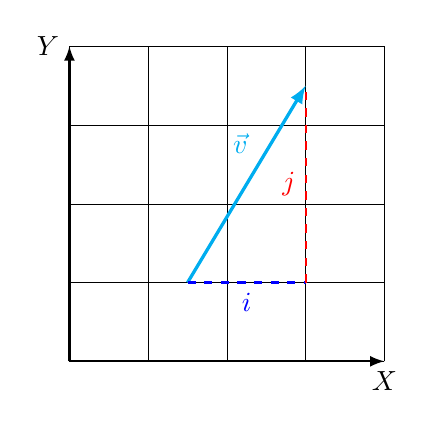
\begin{tikzpicture}
		\draw[step=1, very thin] (0,0) grid (4,4);
		\draw[-latex, thick] (0,0) -- (4,0)
			node[pos=1, below]{$X$};
		\draw[-latex, thick] (0,0) -- (0,4)
			node[pos=1, left]{$Y$};
		\draw[-latex, very thick, cyan] (1.5, 1) -- (3, 3.5)
			node[pos=0.6, above left]{$\vec{v}$};
		\draw[dashed, thick, blue] (1.5, 1) -- (3, 1)
			node[pos=0.5, below]{$i$};
		\draw[dashed, thick, red] (3, 1) -- (3, 3.5)
			node[pos=0.5, left]{$j$};
	\end{tikzpicture}
\end{center}
In questa immagine � possibile vedere un vettore $\mathcolor{cyan}{\vec{v}}(\mathcolor{blue}{i},
\mathcolor{red}{j})$ e le sue componenti.\\[\baselineskip]
D'ora in poi sar� dato per scontato che i vettori siano bi-dimensionali.

\subsection{Operazioni tra vettori}
Le operazioni come addizione e sottrazione funzionano molto semplicemente sommando algebricamente
le componenti tra di loro:
\begin{equation*}
\mathcolor{red}{\vec{v_1}\left(a_1, b_1\right)} \pm 
\mathcolor{blue}{\vec{v_2}\left(a_2, b_2\right)} = 
\mathcolor{purple}{\vec{v}}\left(\mathcolor{red}{a_1}\pm \mathcolor{blue}{a_2}, 
\mathcolor{red}{b_1}\pm \mathcolor{blue}{b_2}\right)
\end{equation*}

La moltiplicazione tra vettori pu� avere come risultato o un \emph{vettore} o uno \emph{scalare}.

\subsubsection{Prodotto scalare}
\begin{equation*}
\mathcolor{red}{\vec{v_1}} \cdot \mathcolor{blue}{\vec{v_2}} = 
\mathcolor{red}{a_1}\mathcolor{blue}{a_2} + \mathcolor{red}{b_1}\mathcolor{blue}{b_2}
\end{equation*}
Come si pu� notare il prodotto scalare tra due vettori torna uno scalare (ovvero un numero).
In fisica per� � molto pi� comune trovare questa definizione di prodotto scalare:
\begin{equation*}
\mathcolor{red}{\vec{v_1}} \cdot \mathcolor{blue}{\vec{v_2}} =
\norm{\mathcolor{red}{\vec{v_1}}}\cdot\norm{\mathcolor{blue}{\vec{v_2}}}\cos\theta
\end{equation*}
$\norm{\vec{v}}$ � il modulo del vettore $\vec{v}$, ovvero la sua lunghezza. $\theta$ � l'angolo
formato dai due vettori.

\subsubsection{Prodotto vettoriale}\label{subsec:vettori:prodottoVettoriale}
\begin{equation*}
\mathcolor{red}{\vec{v_1}} \times \mathcolor{blue}{\vec{v_2}} =
n\norm{\mathcolor{red}{\vec{v_1}}}\cdot\norm{\mathcolor{blue}{\vec{v_2}}}\sin\theta
\end{equation*}
$\norm{\vec{v}}$ � il modulo del vettore $\vec{v}$, ovvero la sua lunghezza. $\theta$ � l'angolo
formato dai due vettori. $n$ � la \emph{normale} del piano su cui stanno i vettori. Una \emph{normale}
� un vettore perpendicolare ad un oggetto dato.\\
Per scoprire la direzione del nuovo vettore si pu� usare la cos� detta 'regola della mano`. Essa dice:
\begin{enumerate}
	\item Usare il pollice della mano destra in direzione e verso del \textbf{primo} vettore
	\item Usare l'indice o le altre dite in direzione e verso del \textbf{secondo} vettore
	\item Il nuovo vettore avr� la direzione che attraversa il palmo perpendicolarmente e il verso 
	uscente dalla mano.
\end{enumerate}